\documentclass[a4paper,11pt,twocolumn]{article}

\usepackage{aas_macros}

\usepackage[utf8]{inputenc}
\usepackage[T1]{fontenc}
\usepackage{lmodern}
%\usepackage{times}
%\usepackage[margin=2cm]{geometry}
\usepackage[a4paper]{geometry}
\usepackage{amsmath}
\usepackage{mathtools}
\usepackage{graphicx}
\usepackage{multirow}
\usepackage{blindtext}
\usepackage{hyperref}
\usepackage{float}
\usepackage{siunitx}

\usepackage{pgfplotstable}
\usepackage{booktabs}
% \pgfplotsset{compat=1.18}


\graphicspath{ {./images/} }

\usepackage[czech]{babel}
\usepackage{graphicx}
\usepackage{amsmath}
\usepackage{xspace}
\usepackage{url}
\usepackage{siunitx}
\usepackage{indentfirst}
\usepackage{subcaption}
\usepackage{caption}
\usepackage{tabularx}
\usepackage{rotating}
\usepackage{tikz}
\usepackage[labelformat=parens,labelsep=quad,skip=3pt]{caption}

\usepackage{color}
\usepackage{listings}

\definecolor{codegreen}{rgb}{0,0.6,0}
\definecolor{codegray}{rgb}{0.5,0.5,0.5}
\definecolor{codepurple}{rgb}{0.58,0,0.82}
\definecolor{backcolour}{rgb}{0.95,0.95,0.92}

\lstdefinestyle{mystyle}{
    backgroundcolor=\color{backcolour},
    commentstyle=\color{codegreen},
    keywordstyle=\color{magenta},
    numberstyle=\tiny\color{codegray},
    stringstyle=\color{codepurple},
    basicstyle=\ttfamily\footnotesize\centering,
    breaklines=true,
    captionpos=b,
    numbers=left,
    numbersep=5pt,
    showspaces=false,
    showstringspaces=false,
    showtabs=false,
    tabsize=2
}

\lstset{style=mystyle}

%\widowpenalty 10000 \clubpenalty 10000 \displaywidowpenalty 10000
\setcounter{topnumber}{3}
\setcounter{bottomnumber}{3}
\setcounter{totalnumber}{6}
\renewcommand\topfraction{0.9}
\renewcommand\bottomfraction{0.9}
\renewcommand\textfraction{0.1}
\intextsep=8mm \textfloatsep=8mm

\renewcommand{\thesection}{\arabic{section}.}
\renewcommand{\thesubsection}{\thesection\arabic{subsection}.}
\makeatletter \def\@seccntformat#1{\csname the#1\endcsname\hspace{1ex}} \makeatother


\begin{document}
    \twocolumn[
    \noindent\hrulefill
    \begin{center}
        \bigskip
        \huge Světelné křivky proměnných hvězd
        \vspace{0.2cm}
        \par \large F4191: Praktikum z astronomie 2
        \par \large Artem Gorodilov
        \vspace{0.2cm}
        \par \large 20. ~prosince 2024
        \bigskip
    \end{center}
    \noindent\hrulefill
    \bigskip
    ]

    \vskip10pt
    \section{Abstrakt}
        V této práci jsem vizualizoval a analyzoval světelné křivky hvězdy WISE J115225.7-665754 (ASASSN-V J115225.64-665753.4 ) se souřadnicemi 11:52:25.73 -66:57:54.2 (178.10721 -66.96506) J2000. 

        Světelné křivky jsem získal z archivních pozorování observatoří TESS a WISE. 
        
        Výpočty byly provedeny pomocí skriptu v Pythonu\textsuperscript{\cite{github}}.
    \section{Úvod}
        Světelné křivky jsou grafy, které znázorňují změny jasnosti hvězdy v čase. U proměnných hvězd, jejichž jasnost se mění periodicky nebo nepravidelně, poskytují světelné křivky klíčové informace o jejich fyzikálních vlastnostech a procesech. Analýza tvaru, amplitudy a periody světelných křivek umožňuje určovat základní parametry hvězd, jako je jejich hmotnost, velikost, teplota nebo fáze evoluce. U binárních hvězd pomáhají identifikovat zatmění a interakce mezi složkami. 

        Pro analýzu světelných křivek je vhodné převést závislost magnitudy/intenzity na čase pozorování na závislost magnitudy na fázi rovnou periodě. 

        \begin{equation}
            \phi = \frac{t \mod P}{P}
        \end{equation}
        
    \section{Zpracování dat}
        \subsection{TESS}
            Data TESS (hlsp\_qlp\_tess\_ffi\_s0065-0000000410922760\_tess\_v01\_llc.fits) byla získána pomocí archivu STScl \textsuperscript{\cite{stsci}}. Data WISE (WISE\ J115225.7-665754\_allwise.ipac a WISE\ J115225.7-665754\_neowise.ipac) byla získána pomocí skriptu wise\_light\_curves.py (Hsiang-Chih Hwang)\textsuperscript{\cite{wise}}. 

            Pozorování TESS bylo provedeno 2023-05-04 05:42:33:33 UT, expozice $\qty{200}{\second}$. Pozorování WISE bylo provedeno dne 2010-01-31 12:21:35:35 UT.  Pozorování WISE je k dispozici jako AllWISE a NeoWISE.

            Pro konstrukci světelné křivky TESS jsem zvolil dobré časové intervaly s parametrem QUALITY > 0. Čas jsem převzal z parametru TIME a tok z parametru SAP\_FLUX. Tok byl normalizován, ale normalizační faktor nebyl uveden. Proto jsem po převodu toku na magnitudu pomocí vzorce (2) získal normalizovanou magnitudu. 

            \begin{equation}
                m = -2.5 \log_{10} F
            \end{equation}

            Dále je třeba vypočítat periodu. K tomuto účelu jsem použil LombScargle z knihovny astropy.timeseries. Nejlepší fit poskytl hodnotu $P = 1.020201 ~\text{d}$. Zatímco data AAVSO dávají hodnotu $P_{\text{AAVSO}}. = 2.0462307 ~\text{d}$. Vhodná hodnota je přibližně poloviční oproti teoretické hodnotě, takže jsem ji vynásobil dvěma $P = 2.040403 ~\text{d}$ a použil obě periody pro výpočet fáze, abych mohl porovnat vizuální výsledky. 

            Pozorování byla prováděna ve filtru TESS s ořezem na $\sim$ 600 nm\textsuperscript{\cite{tess}}.
        
        \subsection{WISE}
            Získání a analýza dat WISE byla mnohem jednodušší než u TESS, protože všechny postupy, které jsem popsal, napsal jeden hezký borec Hsiang-Chih Hwang a zveřejnil přístupnou a jednoduchou dokumentaci na svém GitHubu. 

            Dobré časové intervaly jsem vybral pomocí funkce only\_good\_data\_v1(). Poté jsem získal parametry světelné křivky kombinací dat AllWISE a NeoWISE c pomocí funkce make\_full\_lightcurve\_multibands(). Tentokrát jsem pro výpočet fáze použil pouze teoretickou hodnotu periody. 

            Protože časové jednotky WISE jsou MJD, napsal jsem funkci mjd\_to\_bjd(), která bere souřadnice RA a DEC, čas a převádí je do formátu BJD s odkazem na polohu v Greenwichi. Tato poloha byla zvolena, protože údaje o přesné poloze observatoře se nepodařilo získat. Pro baryocentrickou korekci však bude zcela dostačující.

            Pozorování byla prováděna ve filtru $W1 = 3.4 ~ \mu\text{m}$ (součást čtyřpásmového systému WISE). 
        
        \vspace{10pt}
        K výpočtu veličin a jejich nejistot byla použita knihovna Uncertinties pro Python. Chyby byly rozšířeny o Studentův koeficient (2-Tail Confidence Level) s ohledem na stupně volnosti pro každou hodnotu, pro interval spolehlivosti 68.27\%.

    \section{Vysledky}
        Výsledky jsou uvedeny na obrázcích (\ref{fig:tess_lc_1}), (\ref{fig:tess_lc_2}), (\ref{fig:wise_lc}) a (\ref{fig:lc_comb}).
        
        \begin{figure}
            \centering
            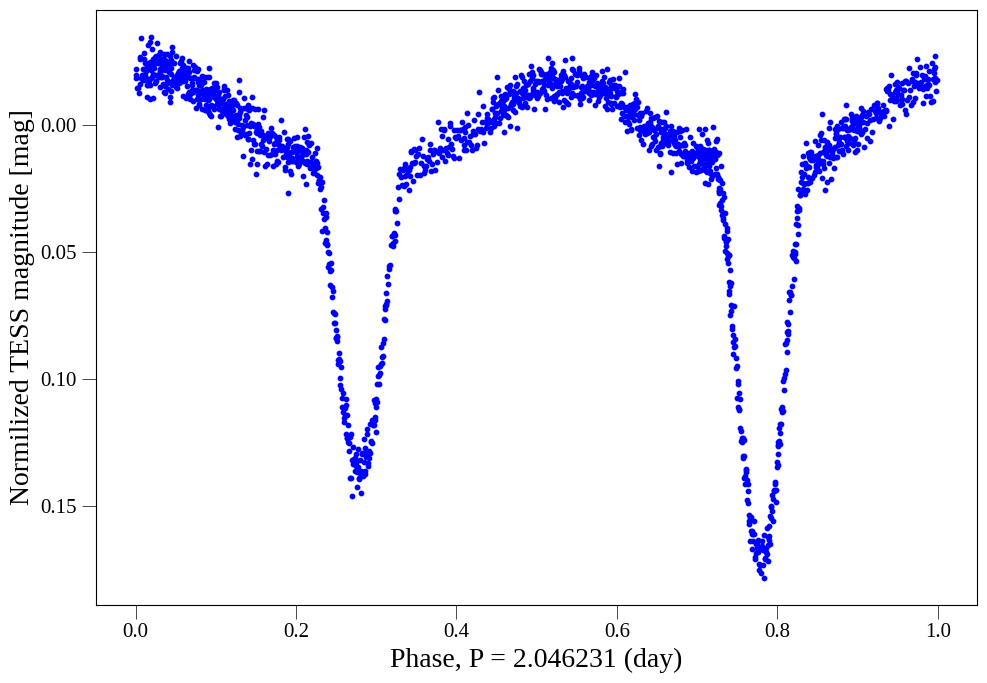
\includegraphics[width=0.5\textwidth]{tess_lc_1.png}
            \caption{Světelná křivka TESS s periodou $P_{\text{AAVSO}}. = 2.0462307 ~\text{d}$}
            \label{fig:tess_lc_1}
        \end{figure}

        \begin{figure}
            \centering
            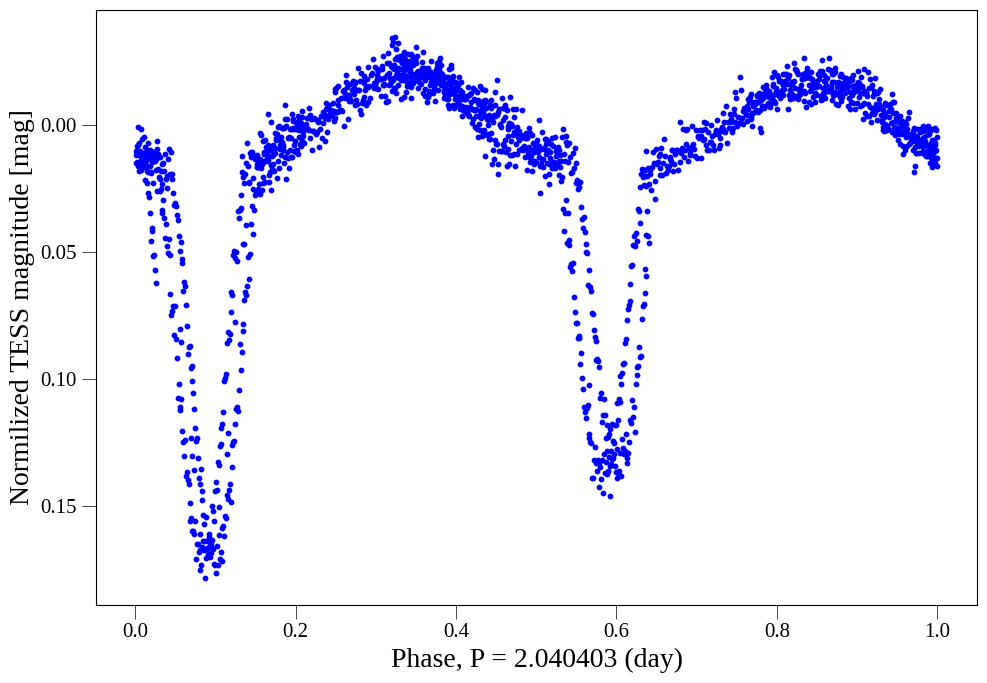
\includegraphics[width=0.5\textwidth]{tess_lc_2.png}
            \caption{Světelná křivka TESS s periodou $P = 2.040403 ~\text{d}$}
            \label{fig:tess_lc_2}
        \end{figure}

        \begin{figure}
            \centering
            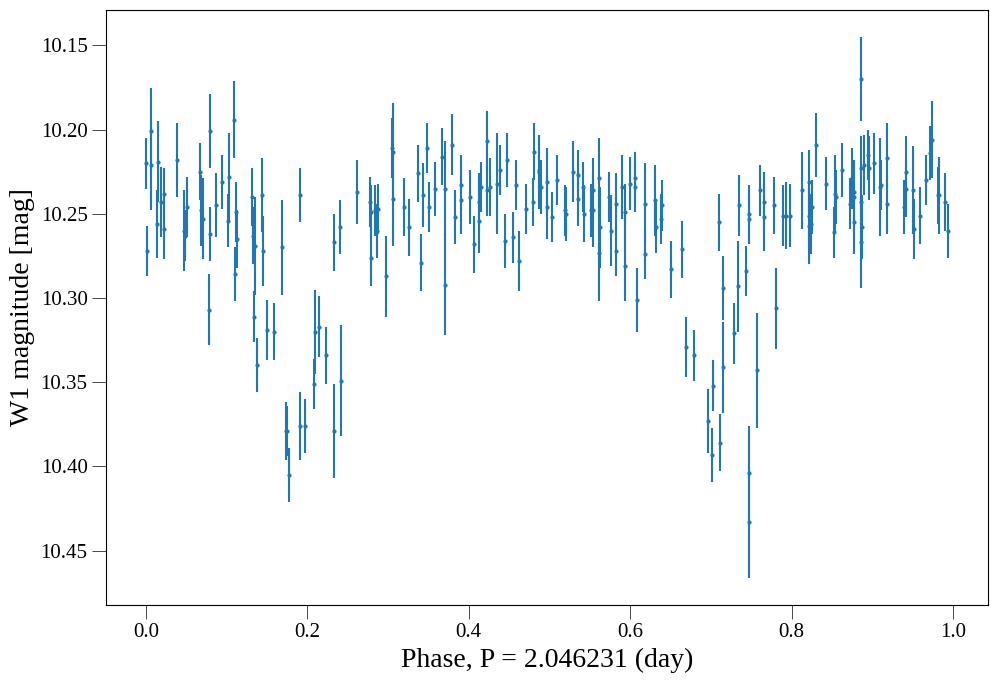
\includegraphics[width=0.5\textwidth]{wise_lc.png}
            \caption{Světelná křivka WISE s periodou $P_{\text{AAVSO}}. = 2.0462307 ~\text{d}$}
            \label{fig:wise_lc}
        \end{figure}

        \begin{figure}
            \centering
            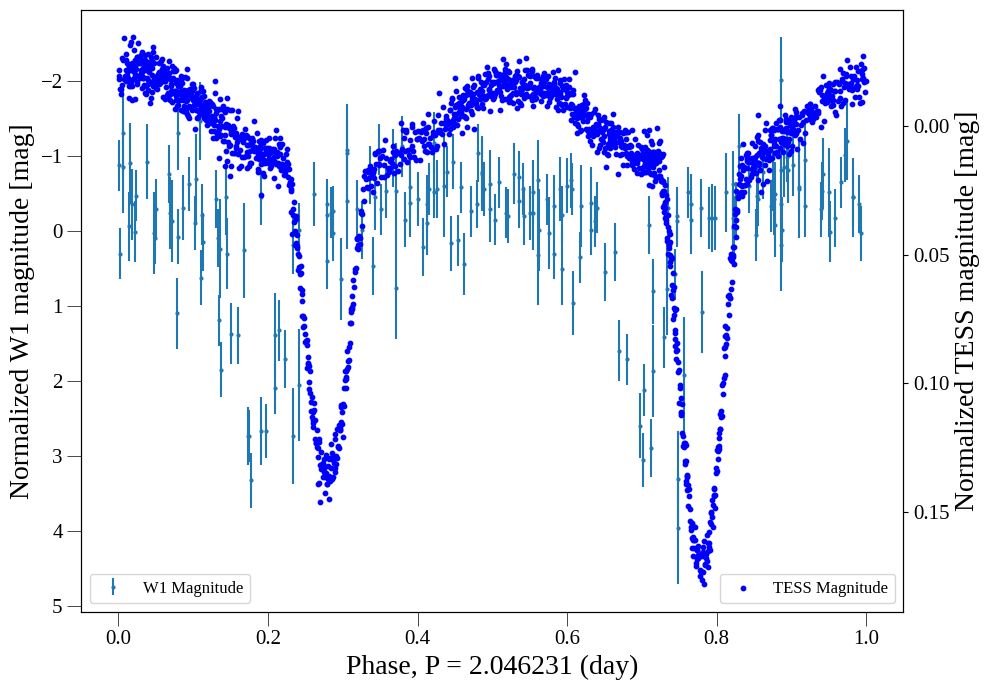
\includegraphics[width=0.5\textwidth]{lc_comb.png}
            \caption{Srovnání světelných křivek TESS a WISE}
            \label{fig:lc_comb}
        \end{figure}

        \begin{figure}
            \centering
            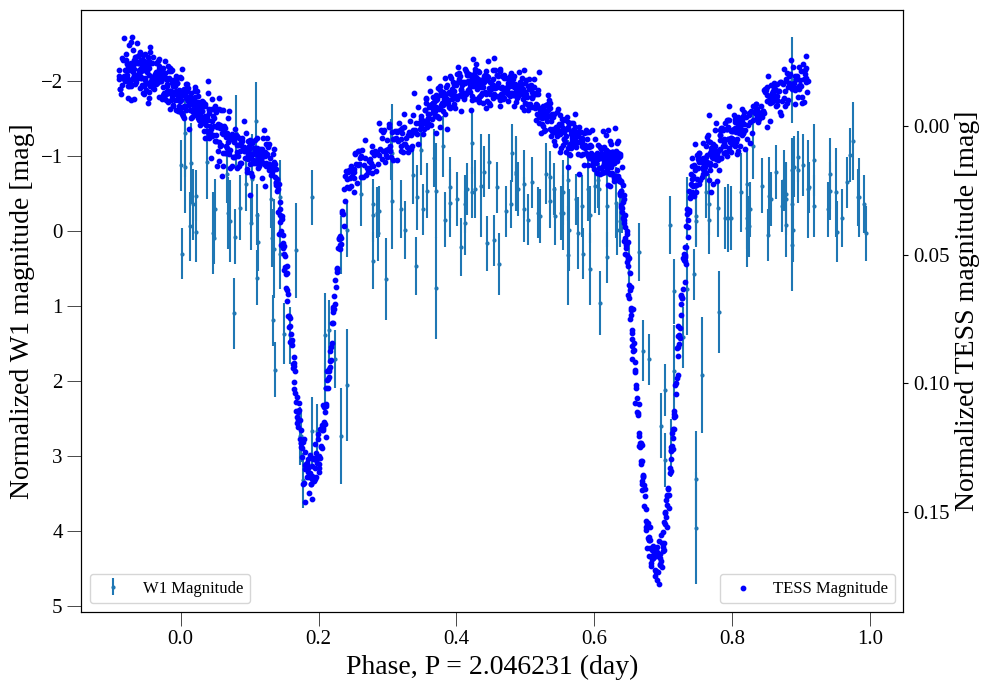
\includegraphics[width=0.5\textwidth]{lc_comb_shift.png}
            \caption{Srovnání světelných křivek TESS a WISE s fázovým posunem 0.09 dne}
            \label{fig:lc_comb_shift}
        \end{figure}

    \section{Závěr}
        Jak je vidět ze světelných křivek pro TESS, fáze získaná z mnou vypočtené periody má rozštěpy v minimech jasnosti, na rozdíl od tvaru křivky pro teoretickou periodu. To svědčí o nepřesnosti vypočtené hodnoty periody (i když rozdíl mezi nimi je pouze 0.005828 d).

        Světelná křivka získaná pomocí WISE má nižší rozlišení než TESS, ale ukazuje stejné fičury ve formě dvou jasnostních minim. 

        Srovnání křivek (viz obr. \ref{fig:lc_comb}) ukazuje, že světelná křivka získaná pomocí TESS má fázový posun přibližně 0,09 dne. Pokud tento posun zohledníme (viz obrázek \ref{fig:lc_comb_shift}), je zřejmé, že tvary křivek s minimy a maximy se navzájem sbližují. Fázový posun může být způsoben několika příčinami. Fázování světelné křivky závisí na zvolené epoše (okamžiku nástupu fáze). Pro data TESS a WISE byly použity různé epochy (BJD, resp. MJD). Chyby v převodu času mohou vést k fázovým posunům. Také rozdílné časové pokrytí dat může ovlivnit určení fáze, pokud byla perioda určena nepřesně. Pokud objekt vykazuje vývoj orbitálních parametrů (např. precesi nebo orbitální migraci), může se skutečná fáze systému s časem měnit.

        Pozorovaná hvězda vykazuje proměnnost odpovídající typu EA\textsuperscript{\cite{vsx}}, která je charakteristická pro zákrytové dvojhvězdy typu Algol. Tyto systémy se skládají ze dvou hvězd, obvykle kulových nebo mírně elipsoidních, které se při pohledu ze Země pravidelně vzájemně zatmívají. Světelná křivka vykazuje zřetelné fáze minimální a maximální jasnosti, přičemž mimo zatmění zůstává jasnost téměř konstantní nebo vykazuje malé změny. Tyto změny mohou být důsledkem reflexních efektů, mírných elipsoidních tvarů hvězd nebo vnitřních změn samotných hvězd. 

        Chtěl jsem také provést fit světelné křivky, ale nedostatečné údaje o systému mi neumožnily použít dostupné modely\textsuperscript{\cite{elisa}}\textsuperscript{\cite{eb}}. Kvůli tomu, že se nepodařilo získat přibližné údaje o teplotách složek systému, jejich hmotnostech, poloměrech a orbitálních parametrech, které fit potřebuje jako výchozí údaje, vede k neadekvátním výsledkům. 

    \bibliographystyle{plain}
    \nocite{*}
    \bibliography{refs/github, refs/stsci, refs/wise, refs/aavso, refs/tess, refs/vsx, refs/elisa, refs/eb}

\end{document}